\chapter{Background}

\label{ch:background}

\section{Workload-Aware Frameworks}

\subsection{Database Cracking}

From Idreos et al., Cracking is a relational database auto-tuning technique which performs online
restructuring of a relational table into disjoint pieces, storing information about each piece within
a separate data-structure called the cracker index.

When a column is queried, it is copied into a version of the column called the cracker column. The
cracker column is then scanned, restructuring it in-place to position the retrieved elements in
contigious positions. The indices of the bounds of the newly formed contigious region are stored
within the cracker index to inform future queries of whether they need to scan that piece of the
column.

Figure \ref{fig:cracking_img} shows two queries being run against a column within a system employing
database cracking. We can see that Q1 partitions copies the column into a cracker column, which is
then partitioned into pieces, of which information is known about the contents. Q2 further breaks
up the column into pieces, and again the information about the newly formed partitions is stored
in the cracker index.

\begin{figure}[h]
  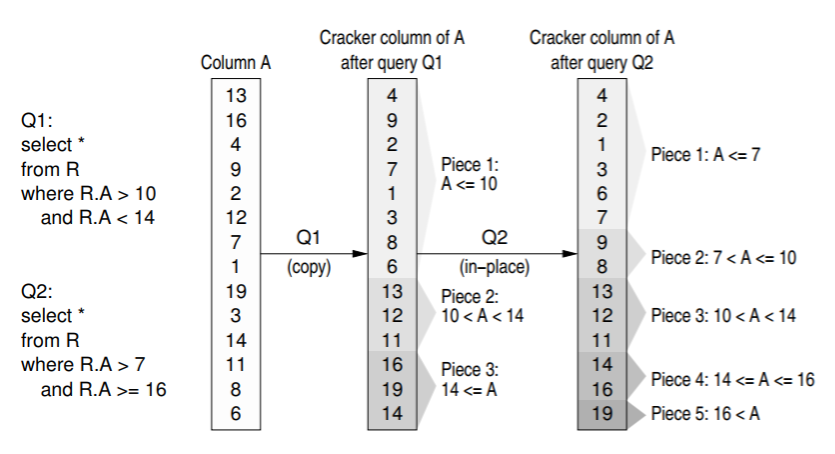
\includegraphics[width=\textwidth]{cracking_img}
  \caption{Illustration of database cracking}
  \label{fig:cracking_img}
\end{figure}

\subsection{Group-by-Query}

In-part inspired by cracking was the thesis work of Aluç, who proposed a group-by-query (G-by-Q)
representation for RDF data, for which the structure of individual database records, as well as
the way records are serialized on the storage system are dynamically determined based on the
workload. This technique proved to be fast and robust against other popular frameworks for
querying RDF data, however, the system is complicated - Aluç's implementation was reported to be
over 35,000 lines of C++. In this work we are aiming to produce simpler contributions.

\section{Frequency Based Clustering}

\section{Graph Algorithms}

\subsection{Breadth First Search}

Breadth first search, or BFS, when run on a graph, involves choosing a starting node as the sole
member of a frontier, which then expands in iterations, wherein members of the frontier add their
out-neighbours which have not yet been visited to the frontier, and remove themselves. This continues
until all vertices have been visited.

There are numerous optimisations which can be made to BFS to improve performance. Storing visited
nodes in a bit-vector provides an effective speed-up, for example. More interestingly, it has been
shown by Beamer et al. that dynamically switching between push and pull iterations can greatly
improve performance on low-diameter, scale free graphs.

The most important factor for us in considering BFS is that it queries the outgoing edges of each
node just once, meaning that the performance gains to be made by an adaptive model are not realised
in the course of a run-through of the algorithm. We use this algorithm to determine what cost there
is to using our adaptive query system when the first query is run, versus a pre-processing system.

\subsection{Pagerank}

Pagerank is a famous algorithm which stores a rank for each vertex and iteratively updates the values
across the entire graph. All nodes are initialised with a rank of $\frac{1}{|V|}$. During each
iteration, each node inherits from all of its in-neighbours a contribution of their pagerank divided
by their out-degree. This value is then multiplied by a damping factor and then added to a base value
to give the updated rank. The base value is defined as $\frac{1 - d}{|V|}$.

In pagerank, every iteration considers all of the vertices and edges in the graph, and so over
an execution of many iterations, any clustering or compression will see further benefits compared to
BFS.

\section{Graph Processing Frameworks}

\subsection{Ligra}

Ligra is a lightweight graph processing framework for shared-memory multi-core machines for graph
traversal algorithms, such as pagerank and BFS. They were in part inspired by Beamer et al.'s work
with shared-memory machines, acheiving speed-up by dynamically switching between push and pull implementations of BFS based on the graph's density. Ligra takes the form of a simple API of two
routines.

